\chapter{DevOps\label{devops}}

DevOps:illa tarkoitetaan ohjelmistokehityksen (engl. \textit{development}) ja IT-toimintojen (engl. \textit{operations}) yhdistämistä. Usein puhutaan sekä DevOps-filosofiasta että DevOps-toimintamallista. DevOps-filosofia keskittyy ohjelmistokehityksen ja IT-toimintojen keinotekoisen jaon välttämiseen ja yhteistoiminnan mahdollistavan kulttuurin rakentamiseen. DevOps-toimintamalli taas keskittyy käytännön toimiin ja teknologioihin, jotka mahdollistavat DevOps-filosofian mukaisen ohjelmistotuotannon. \cite{Klein21}

\section{DevOps-toimintamalli}

DevOps-toimintamalli painottaa jatkuvaa integraatiota ja toimitusta (CI/CD) sekä laadunvalvontaa käyttäen standardisoituja automaattisia menetelmiä. Kuva~\ref{fig:devops} visualisoi DevOps-toimintamallin eri vaiheita. Kehitys- ja operaatiovaiheet tapahtuvat limittäin ja koko prosessi voidaan suorittaa useita kertoja päivässä automatisoidun julkaisuputken avulla. \cite{Jabbari16}

\begin{figure}[ht]
\begin{center}
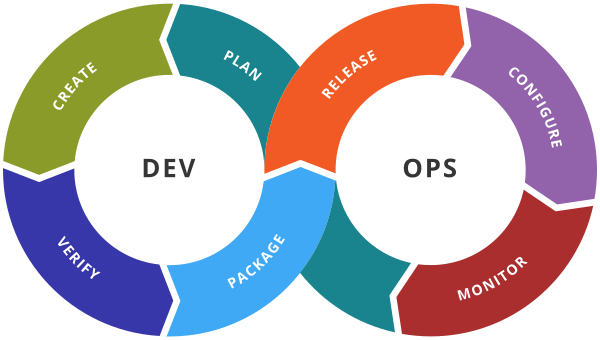
\includegraphics[width=0.6\textwidth]{figures/devops_toolchain.png}
\caption{DevOps-toimintamallin vaiheet.\cite{Wikimedia23}\label{fig:devops}}
\end{center}
\end{figure}

\section{Konttien orkestrointi osana DevOps-toimintamallia}

Konttiteknologiaa käytetään laajasti osana DevOps-toimintamalliin perustuvaa ohjelmistotuotantoa. Konttien mahdollistama alustasta riippumaton ympäristö sallii saman kontin käyttämisen eri vaiheissa DevOps-toimintamallia. \cite{Kang16}

Samalle kontille voidaan ensin suorittaa testit osana jatkuvaa integraatiota. Tämän jälkeen samanlainen kontti voidaan julkaista konttiorkestraatioalustalle, joka huolehtii suorituksessa olevien konttien päivittämisestä uuteen versioon. Konttiorkestraatioalustan tarjoama monitorointi mahdollistaa nopean reaktion ongelmatilanteisiin ja vanha versio kontista voidaan tarvittaessa palauttaa käyttöön nopeasti. \cite{Watada19, Kang16}
